\chapter{Методика исследования}

%В процессе исследовани нами были испытаны грунты методами 
Для определения характеристик переуплотнения грунта, были проведены испытания методом компрессионного сжатия. 

Компрессия "--- способность грунта сжиматься под постоянной, но ступенчато возрастающей нагрузкой без возможности его бокового расширения в условиях открытой системы.

Компрессионное сжатие производилось по ГОСТ 12248-2010 и ГОСТ 15236-2018, в приборах ГТ 1.1.4-01 ООО «НПП ГеоТек» (Пенза) при максимальных ступенях нагрузок до 2.5 МПа на образцах с заданной влажностью. Испытания проводились в двух видах одометров: с диаметром и высотой кольца "--- $72 \times 20$ мм, и $86 \times 25$ мм.
Полученные данные были обработаны методами Казагранде и Беккера. 

 Образцы были поделены на две группы и подготовлены по разным методикам.
 Первая заключалась в достижении заданной влажности и плотности. образцы высушивали, растирали при помощи терки и фарфоровой ступки, а затем с помощью пульверизатора доводили влажность грунтовый массы до необходимого значения влажности. А достижение образца заданной плотности осуществлялось с помощью прибора ПСУ-1.

Вторая методика включала в себя изготовление пасты текучей консистенции. Она заключалась в следующем: образец грунта растирали, а затем водонасыщали до необходимой консистенции. Далее определяли влажность полученной пасты (рис \ref{eq:pst}).


\begin{figure}[ht]
    {\centering
        \subbottom[Загрузка пасты в~компрессионное кольцо]{%
         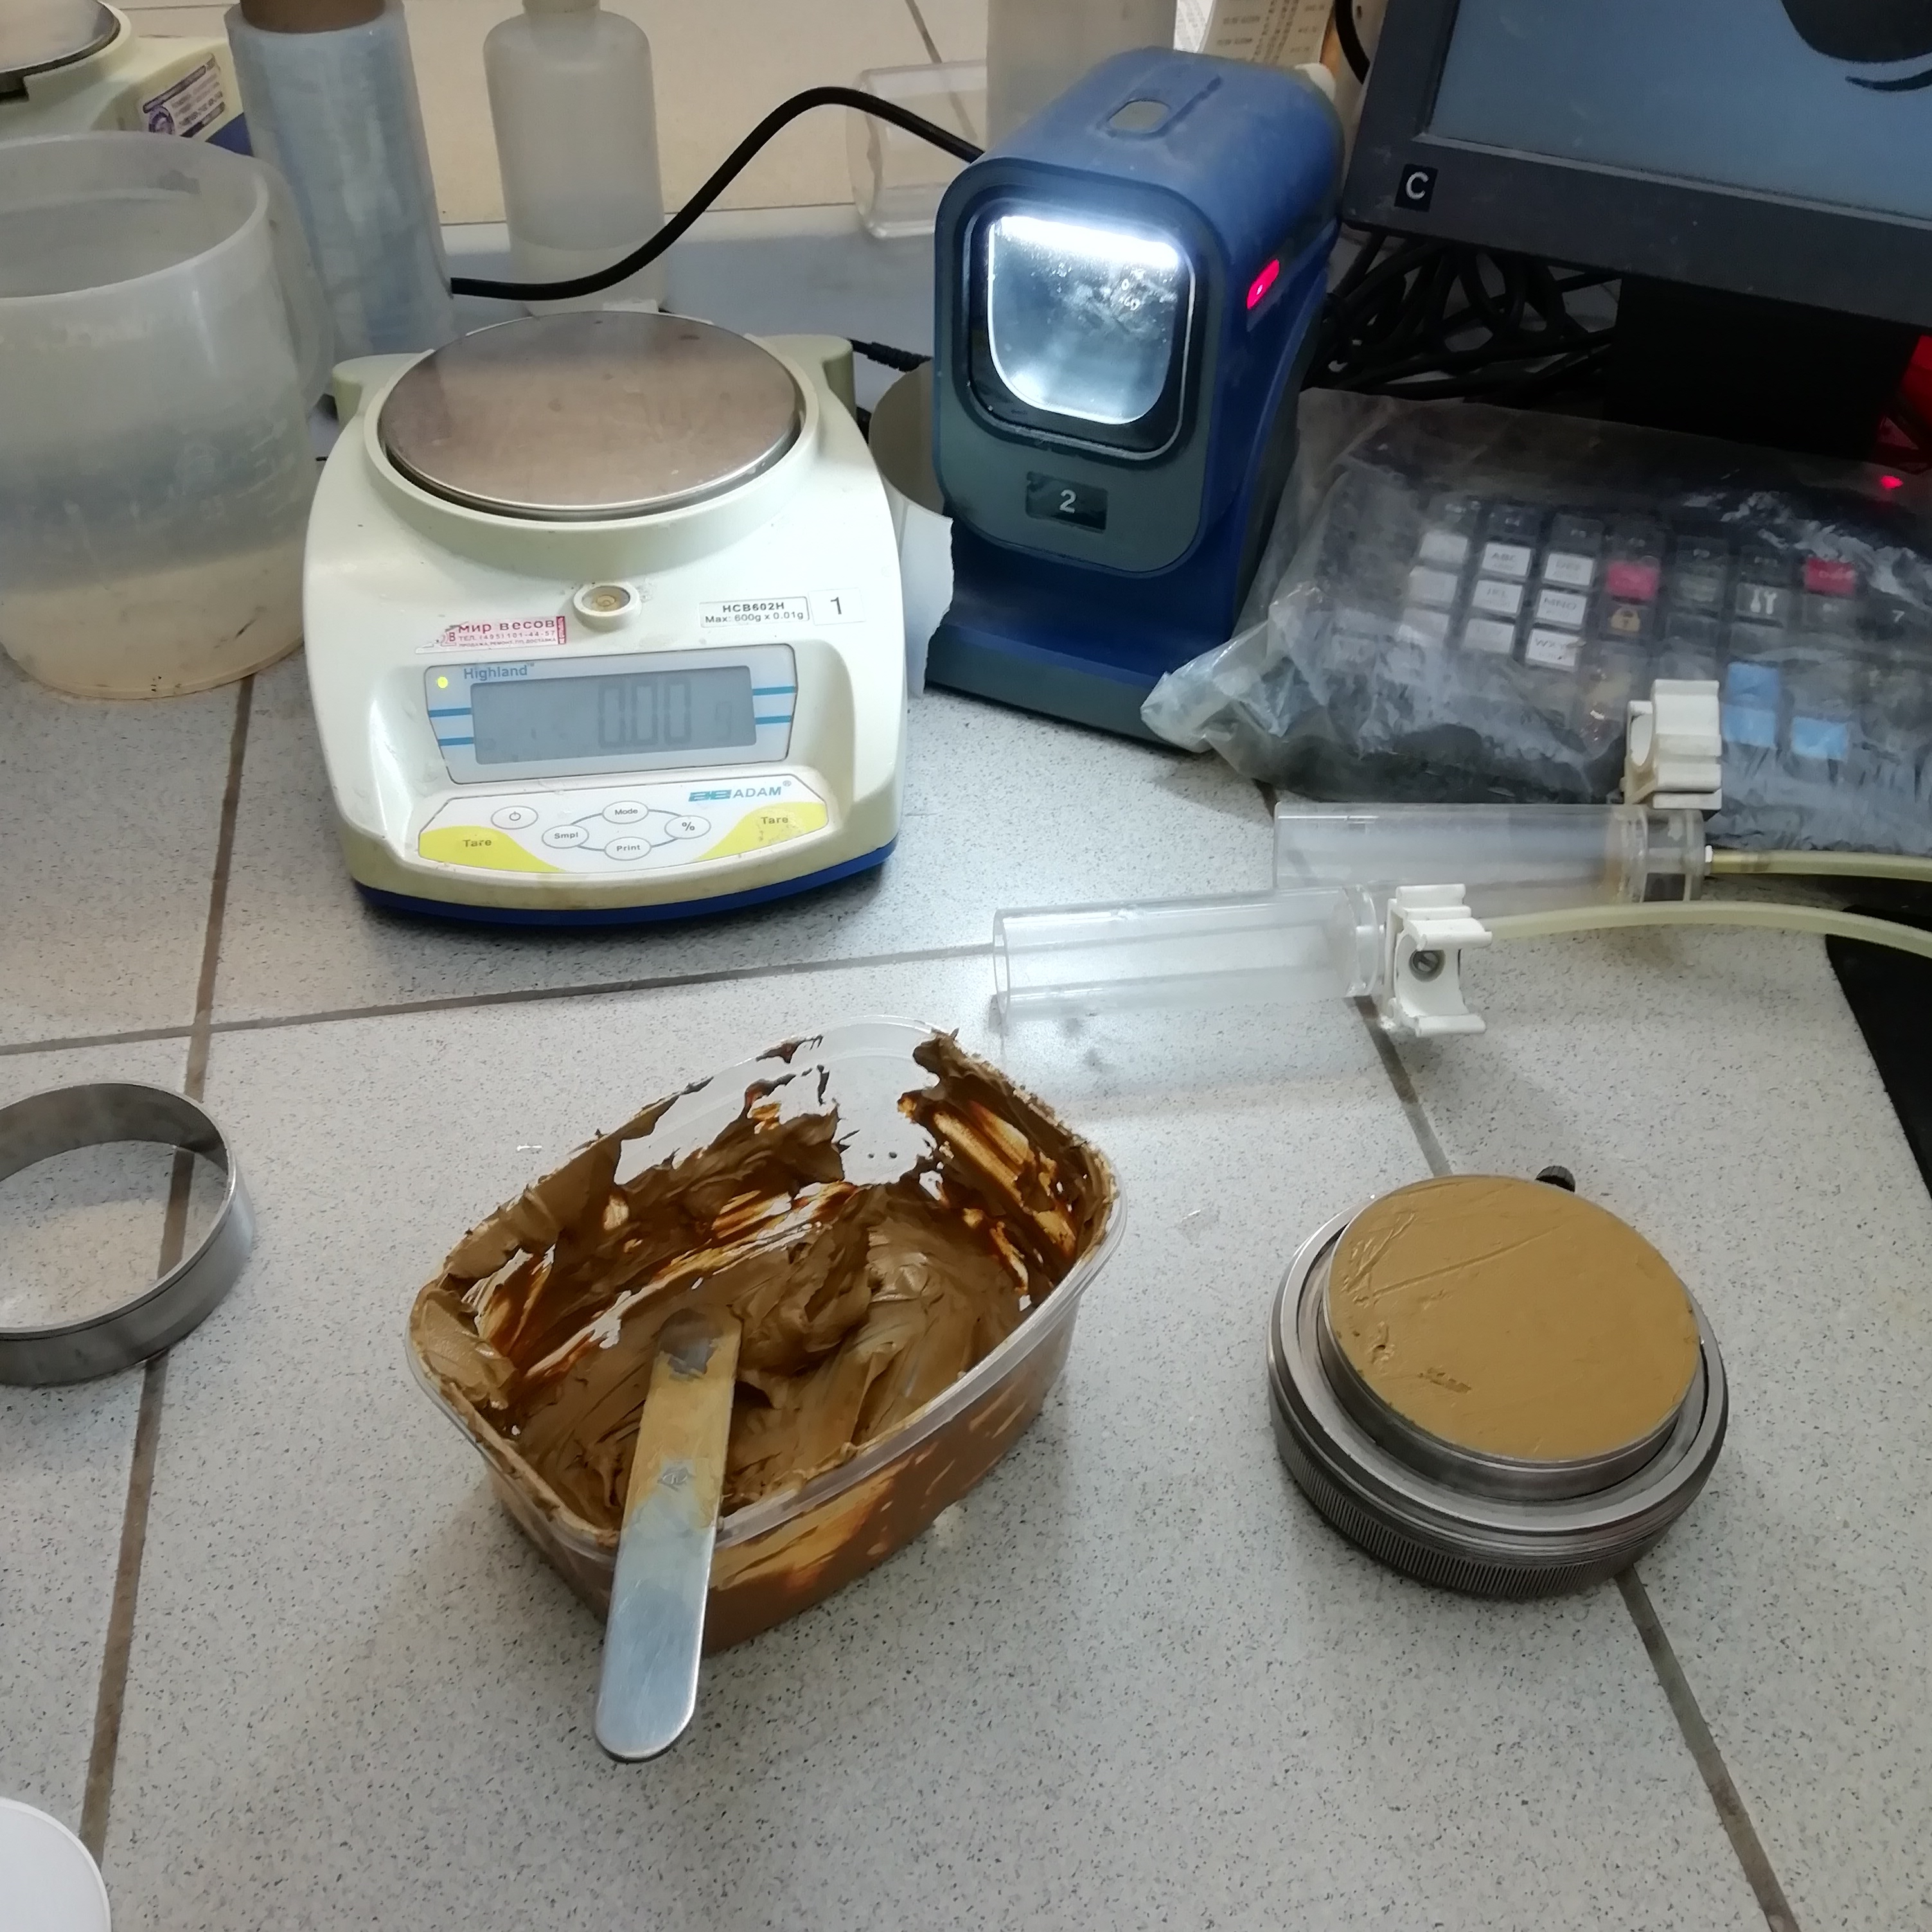
\includegraphics[scale=0.07]{pasta3}}
         \hfill
        \subbottom[Паста загружена в~компрессионное кольцо]{%
          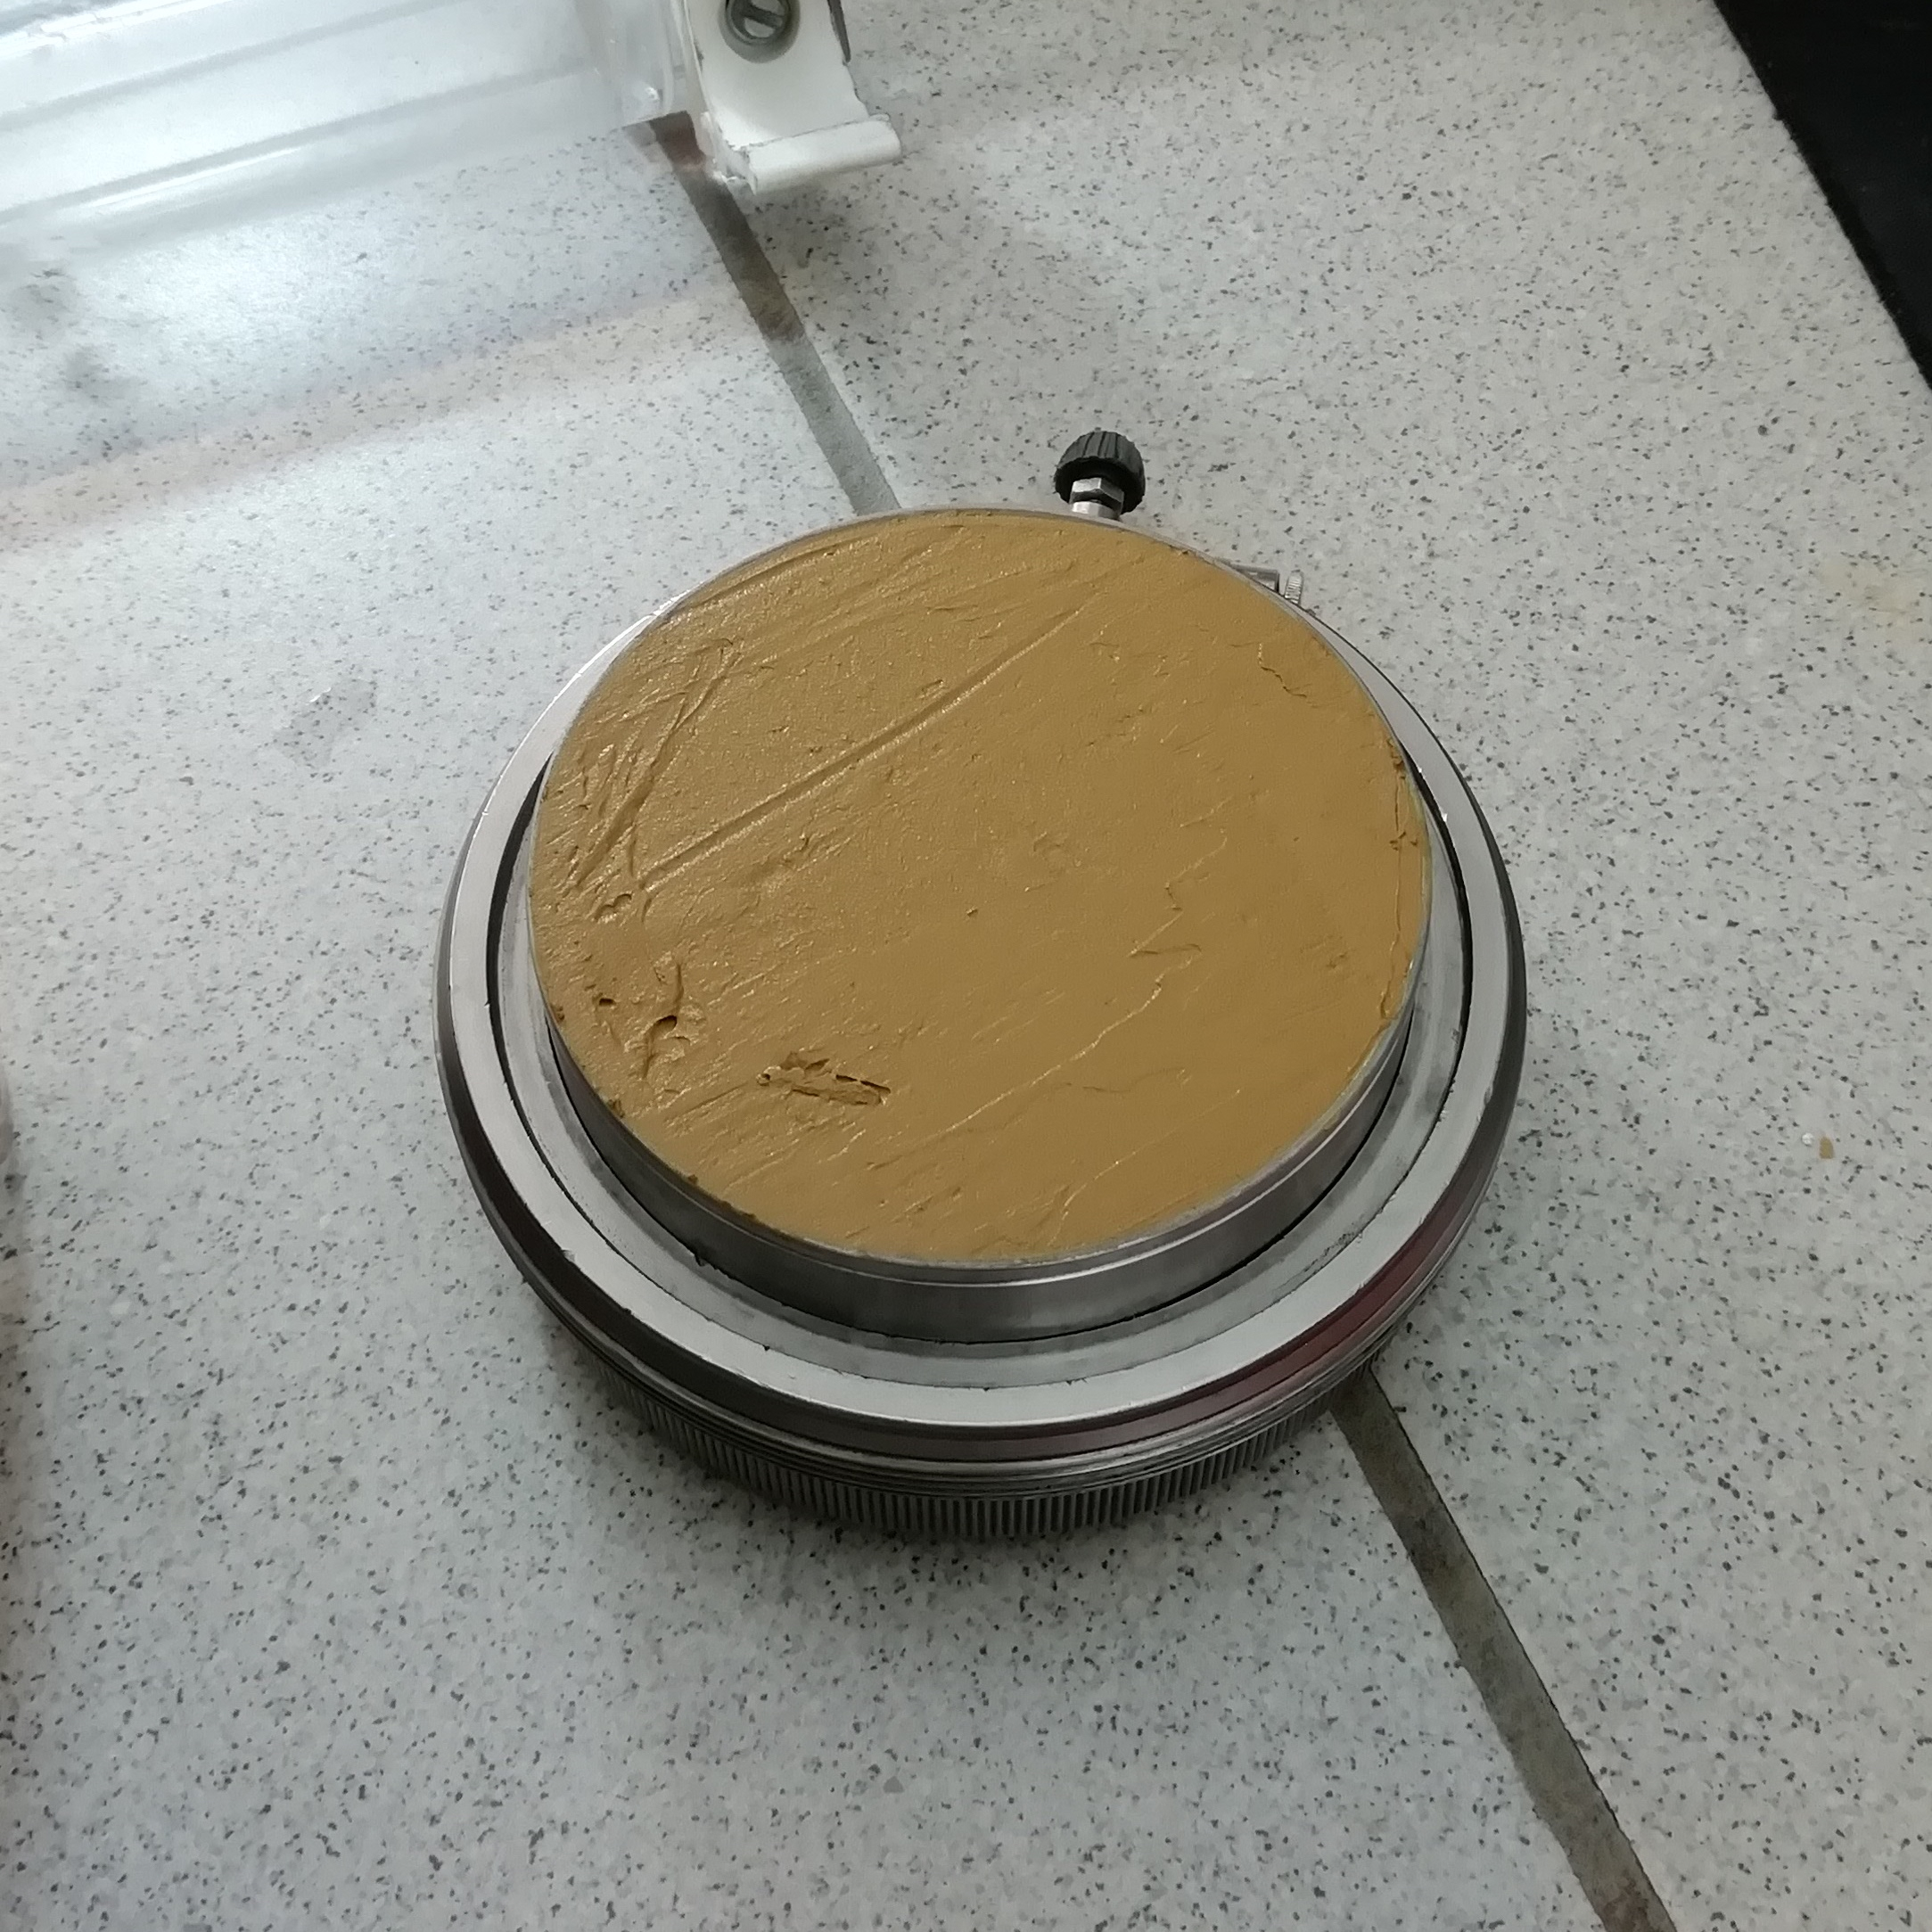
\includegraphics[scale=0.097]{pasta2}}
        \\
        \subbottom[Сборка одометра]{%
          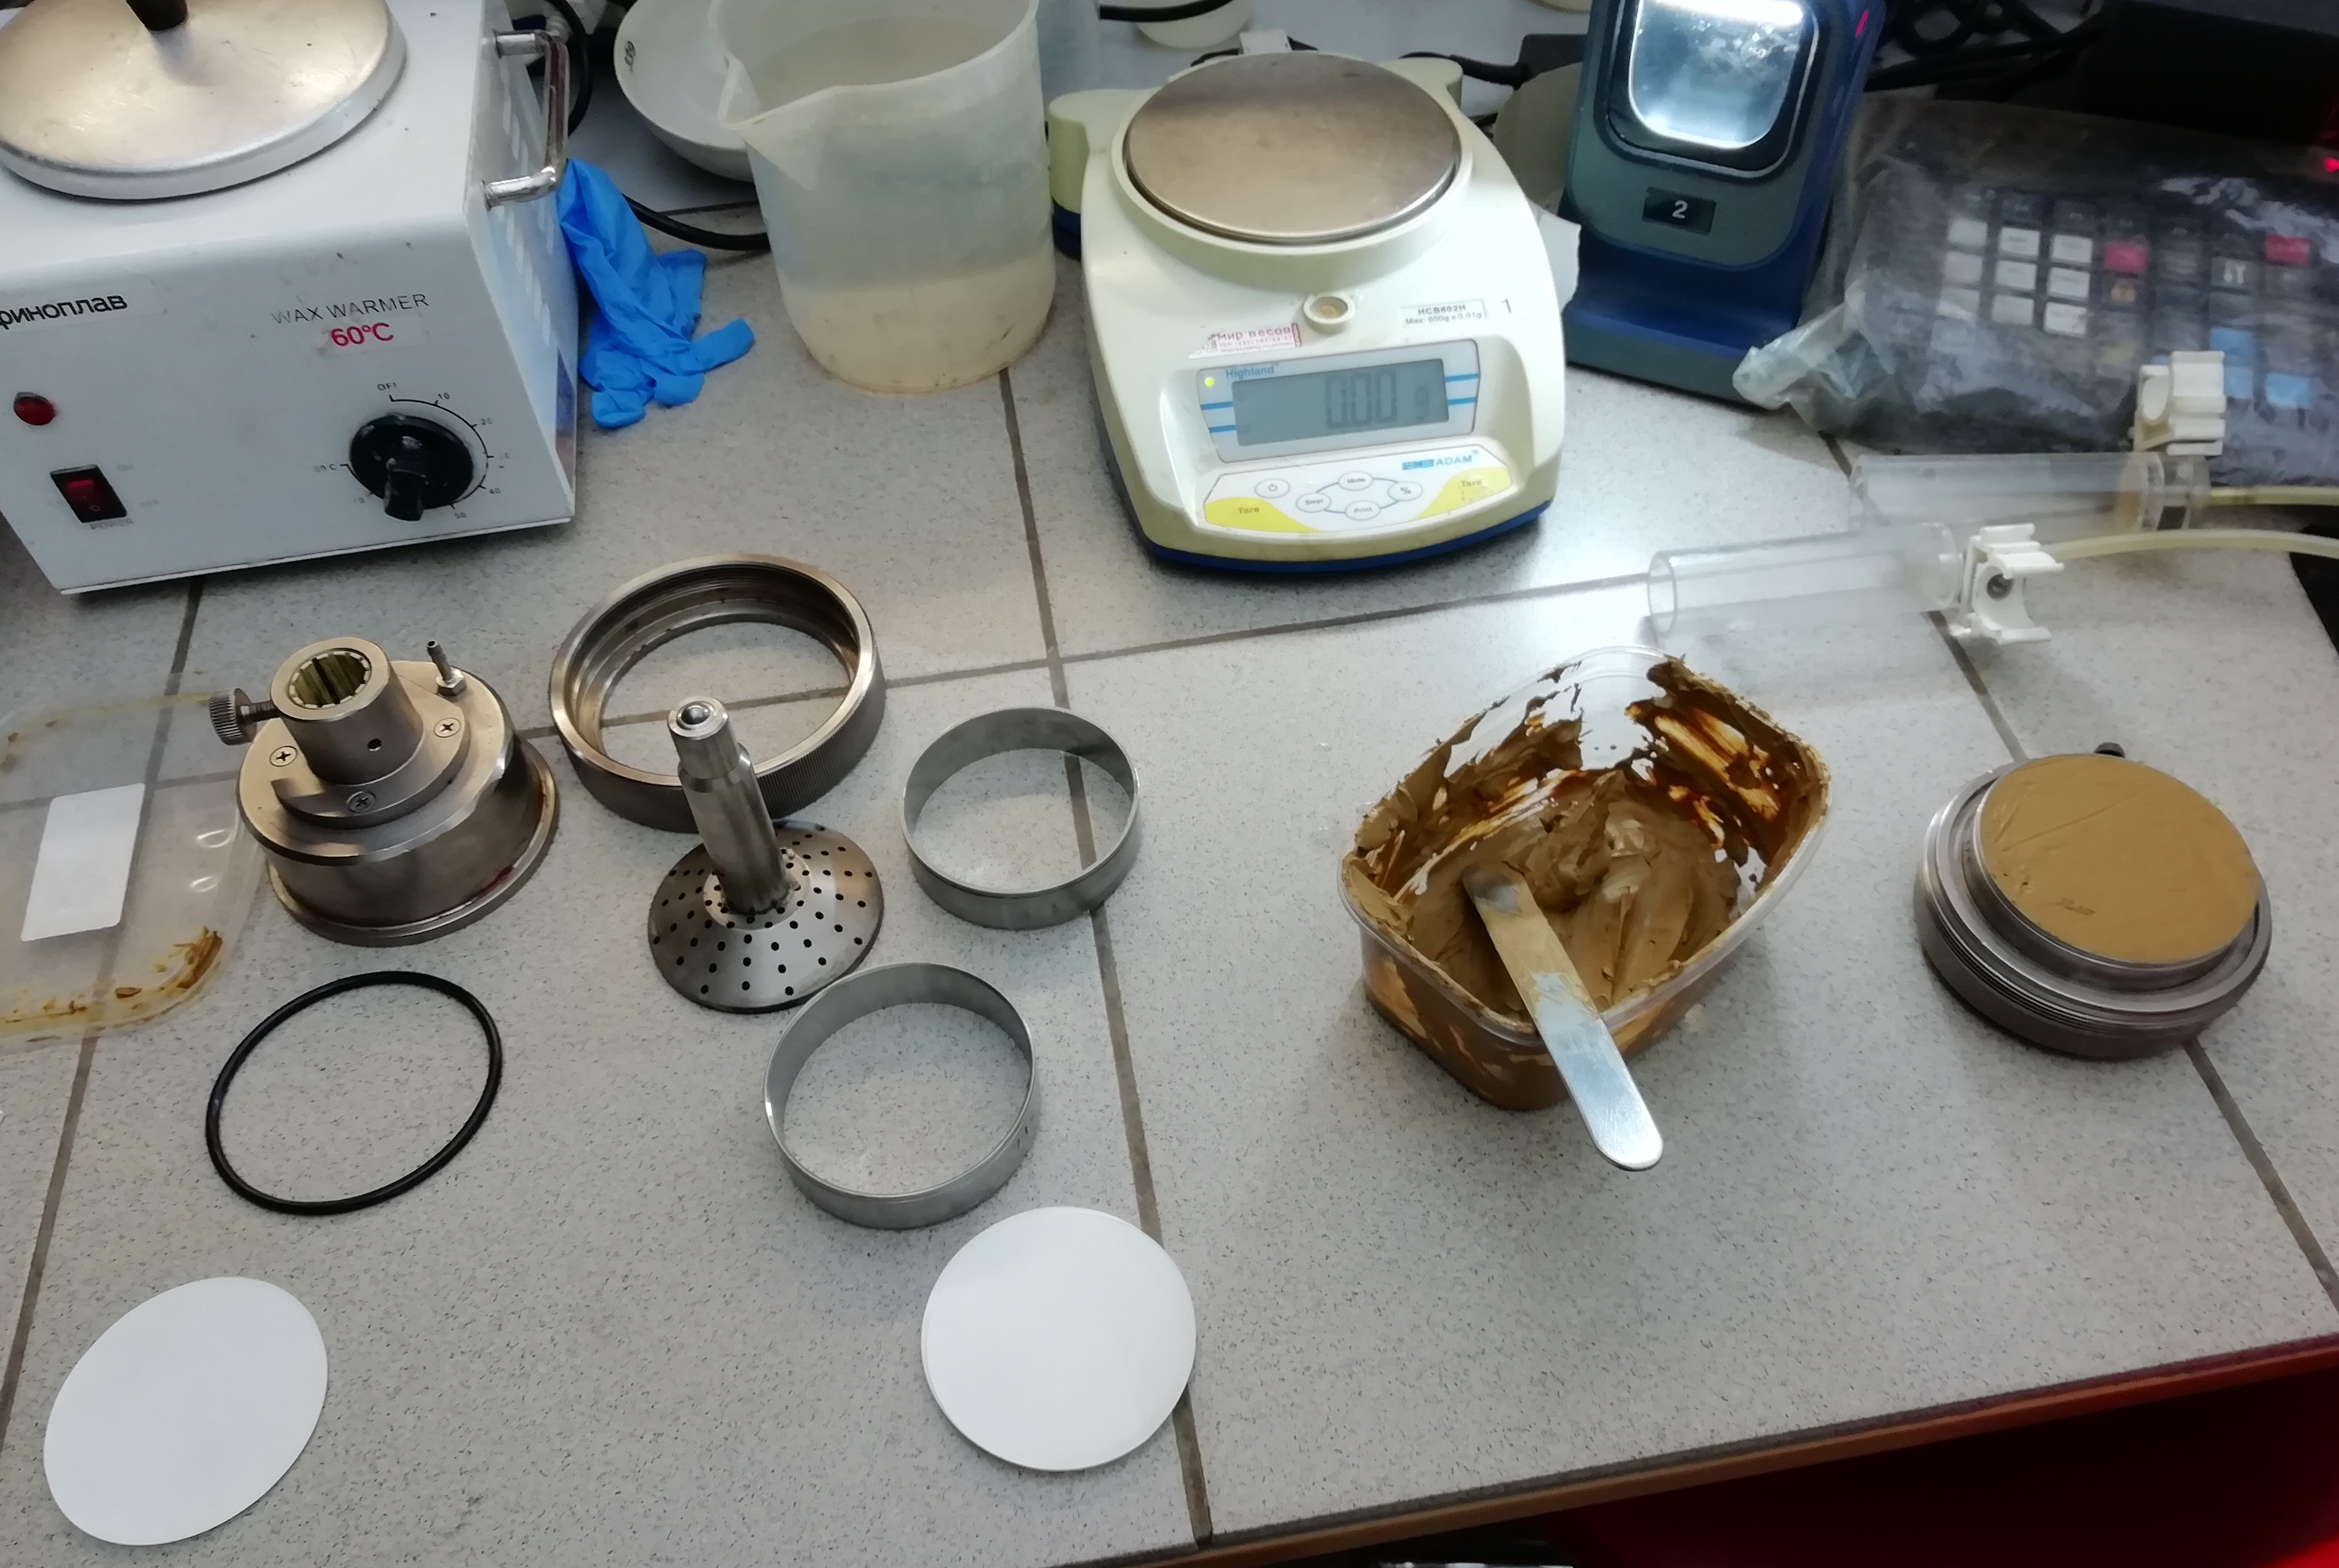
\includegraphics[scale=0.11]{pasta1}}
        \\
    }
    \caption{Подготовка к компрессионным испытаниям}
    \label{eq:pst}
  \end{figure}

\section{Метод Казагранде}

По методу Казагранде строится полулогарифмический график зависимости коэффициента пористости от вертикального напряжения.  
Метод, предложенный Артуром Казагранде, хорошо зарекомендовал себя для глинистых грунтов, однако, графические методы несколько неудобны для инженерного использования.

В логарифмических координатах идеализированная компрессионная кривая в довольно широком интервале вертикальных напряжений представляет собой линейную зависимость в случае непереуплотненного грунта, и билинейную "--- в случае переуплотненного:
первый участок соответствует ветви рекомпрессии, а второй "--- ветви первичного сжатия.

Интуитивно, самым простым способом определения давления предуплотнения, является поиск точки пересечения двух касательных к начальному и конечному участку компрессионной кривой. 
Однако, сложности с выбором касательной к начальному участку кривой, побудили А. Казагранде в 1936 г. создать усовершенствованный метод. 
По-видимому, ученый полагал, что угол наклона касательной заключен в двух крайних положенииях. 
Минимальный угол наклона соответствует горизонтальной прямой, а максимальный "--- углу наклона касательной в точке с наименьшим радиусом кривизны. 
Далее он брал среднее значение этих крайних случаев и проводил биссектрисы между ними. 
Пересечение биссектрисы с касательной конечного участка дает искомую величину напряжения предуплотнения.

По графику компрессионной кривой мы получаем значения вертикальной деформации. Расcчитать величину коэффициента пористостии при данном давлении возможно благодаря формуле, приводящейся в ГОСТ 12248-2010:

$$e_i = e_0 - \epsilon_i (1+e_0),$$

где $e_0$ "--- начальный коэффициент пористости;
$\epsilon_i$ "--- относительная вертикальная деформация грунта.

В этом методе присутствуют сложности, связанные с графическими построениями и наличием субъективного фактора.
Испытания должны быть проведены до таких величин вертикальных напряжений, при которых обеспечивается достоверный выход на линию первичного сжатия. 
Только касательная к такому участку даст единственно верный наклон для построения касательной к конечному участку.
Угол наклона касательной соответствует первой производной в конечной точке.

Точка максимальной кривизны, как правило, выражена не ясно и выбирается геологом субъективно. Для аналитического представления компрессионной кривой точка максимальной кривизны находится для минимума следующей функции:

$$ C(\log \sigma) = \frac{e''(\log \sigma)}{[1+(e'(\log \sigma))^2]^{3/2}}$$

Следующим субъективным фактором является проведение касательной к точке максимальной кривизны, вследствие тех же причин. Это аналитически и по смыслу соответствует значению первой производной компрессионной кривой в этой точке.

Как говорилось ранее, биссектриса является средним значением крайних случаев, а именно минимальным и максимальным углом наклона горизонтальной прямой и касательной в точке с наименьшим радиусом кривизны. 
И таким образом, является оценкой,  осредняющей два крайних значения. 
Помимо этого, построение биссектрисы в пространстве различных размерностей является абсурдным, что приводит к искажениям вследствие выбора масштабов по осям напряжений и коэффициента пористости (Boone, 2010) \cite{boone2010}.

Зависимость от выбранного масштаба  иллюстрируется на рисунке \ref{fig:ellipse}. 
Вместо биссектрисы предлагается использовать линию с угловым коэффициентом в половину от значения первой производной $e' (\log \sigma)$ в точке максимальной кривизны. Это вполне правомерно, потому что эти величины сопоставимы в рамках решаемой задачи:
$$ \tg (\alpha/2) \approx 1/2 \tg (\alpha)$$
Эта величина инвариантна относительно изменения масштаба осей, и при этом гораздо проще вычисляется, что является несомненным преимуществом.



 \begin{figure}
    \center
    \input{Dissertation/images/scale-effect+.pdf_tex}
    \caption{Влияние масштаба осей на результат построения (Clementino, 2005) \cite{clementino2005}}.  \label{fig:ellipse}
\end{figure}
    
\section{Метод Беккера}

Метод Беккера относится к группе энергетических методов.

Согласно методу Беккера, значение напряжения предуплотнения $\sigma_p$ находится по графику зависимости увеличения работы на единицу объема (произведения давления на деформацию) от приращения вертикального давления.
Изменение работы на единицу объема для каждого приращения деформации определяется с помощью формулы \cite{becker1988}:

$$dW = \frac{\sigma_{i-1} + \sigma_i}{2} (\epsilon_{i-1} - \epsilon_i)$$
\begin{itemize}
    \item $dW$ "--- изменение работы на единицу объема 
    \item $\sigma_{i-1}$ "--- напряжение предыдущей ступени нагружения кПа;
    \item $\sigma_i$ "--- напряжение текущей ступени нагружения кПа;
    \item $\epsilon_{i-1}$ "--- относительная деформация, достигнутая на предыдущей ступени нагружения, д.\:е.;
    \item $\epsilon_i$ "--- относительная деформация, достигнутая на текущей ступени нагружения, д.\:е.
\end{itemize}

В своей работе Беккер указывает, что величина давления, равного суммарной работе, определяется давлением в конце приращения деформации. 
Полученная зависимость, как правило, имеет два прямолинейных участка. 
Напряжение, соответствующее точке пересечения двух прямых, проведенных к линейным участкам кривой, соответствует давлению предварительного уплотнения (D.Becker at all, 1988) \cite{becker1988}.

Вследствие эквивалентности пространства построения $W - \sigma$ эквивалентно пространству $e - \ln \sigma$, что подтверждается следующим уравнением (Wang, 2004) \cite{wang2004}: 

$$de = C_c d \log\sigma$$
$$dE = \int_{\sigma_1}^{\sigma_2} \frac{\sigma}{1+e_0} de 
= \int_{\sigma_1}^{\sigma_2} \frac{\sigma}{1+e_0} \frac{C_c d\sigma}{\sigma}
= \frac{C_c (\sigma_2 "--- \sigma_1)}{1+e_0}$$


Соответственно, к недостаткам метода, так же как и для метода Казагранде, можно отнести наличие субъективного фактора при графических построениях, в частности сложность в выборе линейных участков, к которым проводятся прямые.

В зависимости от типов грунтов, тот или иной метод может оказаться чувствительнее, поэтому в ГОСТ 58326-2018 рекомендуется проводить обработку результатов всегда двумя способами и выбирать из них меньшее значение переуплотнения, то есть то, которое обеспечивает наибольший запас при проектировании.

Метод Беккера является не единственным энергетическим методом, которые использовались и используются в настоящее время. Существуют и работы предшественников, например, энергетический метод, показанный норвежским ученым Tavenas. В методе график зависимости напряжения от деформации используют непосредственно на основе кривой компрессии без учета перезагрузочной части испытания. Для более консолидированных образцов, график напряжения/деформации состоит из двух частей: первая часть кривой возрастает более резко, чем вторая. Точка пересечения двух линий, определяется как давление предварительного уплотнения (Tavenas, 1979) \cite{tavenas1979}.

\section{Подготовка и проведение испытаний}

Для проведения испытаний были подготовлены образцы нарушенного сложения из грунтов, отобранных на месте изысканий (скв. 26, 27, 38, 39). Грунтовая паста доводилась до текучего состояния с влажностью превышающей в 1,5--2 раза влажность на пределе текучести. 
Паста текучей конситенции использовалась с целью представления образца нормально уплотненного грунта.

Испытания проводились в два этапа.
Схема испытаний для первого этапа была составлена таким образом, чтобы смоделировать процесс седиментации образца, достижения им заданного максимального исторического давления, процесса извлечения образца на поверхность.

Второй этап моделировал собственно компрессионное сжатие образца в одометре, после его извлечения из массива грунта.

Для этого грунтовая паста нагружалась ступенями начиная с 6 кПа.
Каждая последующая ступень принималась в два раза больше предыдущей.
Максимальное напряжение по первой ветви нагрузки соответсвовало 600 кПа.
Первая ветвь нагружения соответствует ветви первичной компрессии.

Затем проводилась постепенная полная разгрузка образца.

После этого образец нагружался по схеме первой ветви, но до максимального давления 2500 кПа.
Цель работы была найти перегиб на второй ветви, соответствующей переходу образца из зоны рекомпрессии в зону первичного сжатия.
Такой последованностью действий возможно показать всю историю нагрузок и подробно воссоздать природные наряжения, при которых существовал грунт. 

Как говорилось ранее, в данной работе рассматривается единственный фактор: максимальное историческое напряжение. Поэтому для того, чтобы оценить точность методов Казагранде и Беккера, грунты нарушенной структуры были испытаны по данной схеме, что не противоречит ГОСТ 58326-2018.

Так же одной из промежуточных задач работы было определение коэффициента вторичной консолидации, поэтому испытания получились достаточно длительными. Этот коэффициент применяется для расчета напряжения предуплотнения грунтов методом Thogersen, который не вошел в данную работу.
 
